%%%%%%%%%%
%
% DIRECTIONS
% Students count off 1, 2, 3, ..., 7
% Then each does that number (or takes a guess)
% Then explains their answer to their neighbor
% Volunteers write their answers on a copy
%   under a document camera.
%
%%%%%%%%%%

\RequirePackage{luatex85}
\documentclass[10pt, addpoints]{exam}
\usepackage{tikz, pgfplots, amsmath, mathtools, multicol}
\usepackage[letterpaper, landscape, margin=0.5in, column sep=1in]{geometry}
\setlength\parindent{0mm}

\usepackage{expl3}
\ExplSyntaxOn
\cs_new_eq:NN \Repeat \prg_replicate:nn
\ExplSyntaxOff

\newcommand\diagram{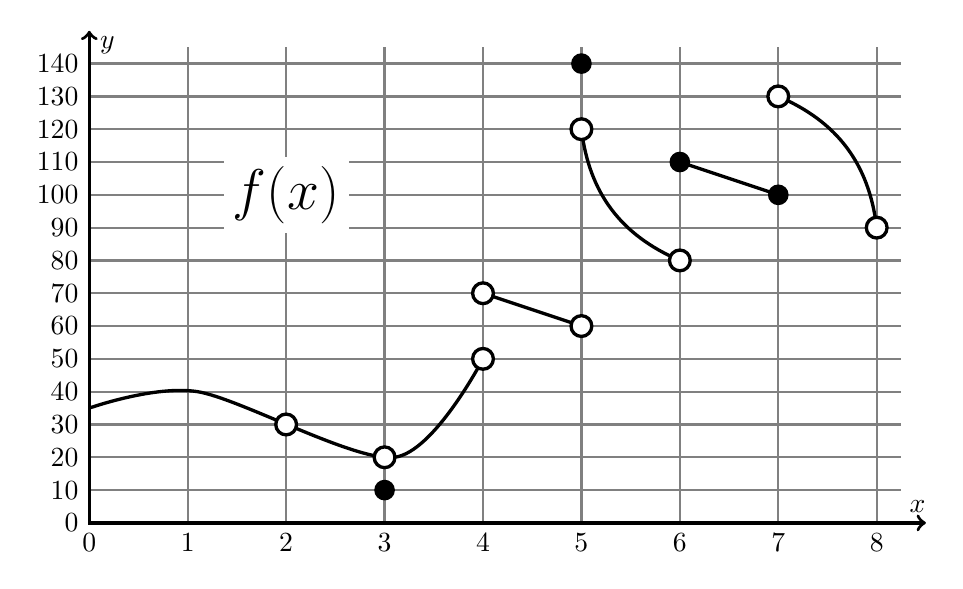
\begin{tikzpicture}
		[scale=1.25, very thick]
	\draw[gray, thick, yscale=1/3] (0,0) grid (8.25,14.5);
	\draw[<->] (0,15/3) -- node[pos=0.03, right] {$y$} (0,0) --  node[pos=0.99, above] {$x$} (8.5,0);
	\foreach \y in {0,10,...,140}
	\draw (0,\y/30) node[left] {\y};
	\foreach \x in {0,...,8}
	\draw (\x,0) node[below] {\x};
	%\draw[rounded corners=10] (0,2/3) -- (1,1) -- (2,2/3) -- (3,1/3) -- (4,5/3);
	\draw[smooth] plot coordinates{(0,3.5/3) (1.1,4/3) (3.1,2/3) (4,5/3)};
	\draw (4,7/3) -- (5,6/3);
	\draw (5,12/3) to [bend right=30] (6,8/3);
	\draw (6,11/3) -- (7,10/3);
	\draw (7,13/3) to [bend left=30]  (8,9/3);
	\foreach \x/\y in {2/3, 3/2, 4/5, 4/7, 5/6, 5/12, 6/8, 7/13, 8/9}
	\draw[black, fill=white] (\x,\y/3) circle (3pt);
	\foreach \x/\y in {3/1, 5/14, 6/11, 7/10}
	\draw[black, fill=black] (\x,\y/3) circle (2.5pt);
	\draw (2,10/3) node[fill,white] {\color{black} \huge$f(x)$};
	\end{tikzpicture}}

\newcommand\content[5]{\question $\left\{\begin{aligned}
	\phantom{\lim_{x\to \mathbf{#1}^+}} f(#1) &= #2
	\\[-0.5ex] \lim_{x\to \mathbf{#1}^-}f(x) &= #3
	\\[-0.5ex] \lim_{x\to \mathbf{#1}^+}f(x) &= #4
	\\[-0.5ex] \lim_{x\to \mathbf{#1}\phantom{^+}}f(x) &= #5
	\end{aligned}\right.$}

\thispagestyle{empty}
\pagestyle{empty}
\begin{document}
\begin{multicols}2
\Repeat{1}{
	{\large Name:} \hfill \underline{\hspace{4in}} 
	\par\bigskip
	\diagram
	\par\vfill
	\begin{multicols}{2}
	\begin{questions}
	\content1{}{}{}{}
	\content2{}{}{}{}
	\content3{}{}{}{}
	\content4{}{}{}{}
	\content5{}{}{}{}
	\content6{}{}{}{}
	\content7{}{}{}{}
	\end{questions}
	\end{multicols}
	}

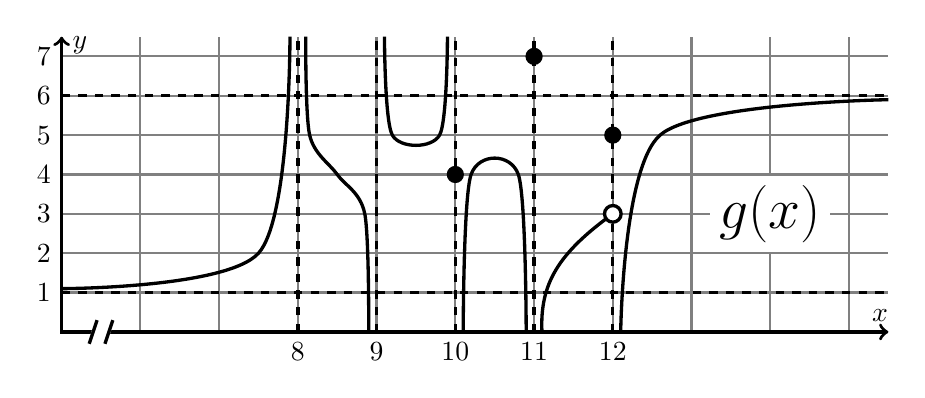
\begin{tikzpicture}
		[very thick,yscale=0.5]
	\draw[gray, thick, yscale=1] (5,0) grid (15.5,7.5);
	\foreach \x in {8,...,12}
	\draw[dashed] (\x,0) -- (\x,7.5);
	\foreach \y in {1,6}
	\draw[dashed] (5,\y) -- (15.5,\y);
	\draw[<->] (5,7.5) -- node[pos=0.03, right] {$y$} (5,0) --  node[pos=0.99, above] {$x$} (15.5,0);
	\foreach \y in {1,...,7}
	\draw (5,\y) node[left] {\y};
	\foreach \x in {8,...,12}
	\draw (\x,0) node[below] {\x};
	\draw[fill, white] (5.45-0.1,-0.3) -- ++(right:0.2) -- ++(0.1,0.6) -- ++(left:0.2) -- ++(-0.1,-0.6);
	\draw (5.45-0.1,-0.3) ++(right:0.2) -- ++(0.1,0.6) ++(left:0.2) -- ++(-0.1,-0.6);
%	\draw[rounded corners=20] (5,1) -- (6,1) -- (6,7.5);
	\draw[smooth] plot coordinates {(5,1.1) (7.5,2) (7.9,7.5)};
	\draw[smooth] plot coordinates {(8.1,7.5) (8.15,5) (8.5,4) (8.85,3) (8.9,0)};
	\draw[smooth] plot coordinates {(9.1,7.5) (9.2,5) (9.8,5) (9.9,7.5)};
	\draw[smooth] plot coordinates {(10.1,0) (10.2,4) (10.8,4) (10.9,0)};
	\draw (11.1,0) to [bend left=18] (12,3);
	\draw[smooth] plot coordinates {(12.1,0) (12.6,5) (15.5,5.9)};
	\foreach \x/\y in {12/3}
	\draw[black, fill=white,yscale=2] (\x,\y/2) circle (3pt);
	\foreach \x/\y in {12/5, 11/7, 10/4}
	\draw[black, fill=black,yscale=2] (\x,\y/2) circle (2.5pt);
	\draw (14,3) node[fill,white] {\color{black} \huge$g(x)$};
	\end{tikzpicture}

\renewcommand\content[5]{\question $\left\{\begin{aligned}
	\phantom{\lim_{x\to \mathbf{#1}^+}} g(#1) &= #2
	\\[-0.5ex] \lim_{x\to \mathbf{#1}^-}g(x) &= #3
	\\[-0.5ex] \lim_{x\to \mathbf{#1}^+}g(x) &= #4
	\\[-0.5ex] \lim_{x\to \mathbf{#1}\phantom{^+}}g(x) &= #5
	\end{aligned}\right.$}

\begin{multicols}{2}
	\begin{questions}
	\setcounter{question}7
	\content8{}{}{}{}
	\content9{}{}{}{}
	\content{10}{}{}{}{}
	\content{11}{}{}{}{}
	\content{12}{}{}{}{}
	\bigskip
	\question $\lim\limits_{x\to \mathbf{-\infty}}g(x) =$
	\question $\lim\limits_{x\to \mathbf{+\infty}}g(x) =$
	\end{questions}
	\end{multicols}
\end{multicols}

\clearpage
\newcommand{\gaacard}[4]{
\question $
%\begin{minipage}[c][1.1 in]{0.99in}{
%\begin{center}
\begin{matrix}
\begin{tikzpicture}
\begin{axis}[
    every axis/.append style={font=\tiny}, 
   	xmin=-3.1, xmax=3.1,
	ymin=-2.5, ymax=2.5,
	samples=99, 
	major tick length={0},
	line width=1pt,
 	axis lines=center, height=2.2in, width=2.2in, grid=major,
 	restrict y to domain=-2.5:2.5, 
%	title={\normalsize{\unboldmath$\displaystyle f(x) = #1$}},
	extra y tick style={y tick label style={right}},
	#3
	]
    \addplot [black, smooth, thick, domain=-3:3] {#2};
    #4
\end{axis}
\end{tikzpicture}
\end{matrix}
%\end{center}}
%\end{minipage}
\,\,
\begin{aligned}
	\phantom{\lim_{x\to \mathbf0^+}} f(x) &= \smash{#1}
	\\[-0.9ex] \phantom{\lim_{x\to \mathbf0^+}} f(0) &=
	\\[-0.9ex] \lim_{x\to \mathbf0^-}f(x) &=
	\\[-0.9ex] \lim_{x\to \mathbf0^+}f(x) &=
	\\[-0.9ex] \lim_{x\to \mathbf0\phantom{^+}}f(x) &=
	\\[-0.9ex] \lim_{x\to \mathrlap{-\infty}\phantom{\mathbf0{^+}}}f(x) &=
	\\[-0.9ex] \lim_{x\to \mathrlap{+\infty}\phantom{\mathbf0{^+}}}f(x) &=
	\end{aligned}
$ \par\bigskip\bigskip}
\newcommand\gacard[3]{\gaacard{#1}{#2}{#3}{}}
\newcommand\gcard[2]{\gacard{#1}{#2}{grid=none, ticks=none}}
\newcommand\opencircle[1]{\draw[color=black,fill=white,thick] (axis cs:{#1}) circle [radius=2pt];}

\setlength\columnsep{0mm}
\begin{multicols}3
	\begin{questions}
	\setcounter{question}{14}
	\gcard{1/x}{1/x}
	\gcard{1/x^2}{1/x/x}
	\gcard{x^2}{x^2}
	\gcard{x^3}{x^3}
	
	\gacard{e^x}{e^x}{ytick={1}, xtick={0}}
	\gacard{\ln(x)}{ln(x)}{ytick={0}, xtick={1}}
	
%	\columnbreak
	\gaacard{\frac{\left| x \right|}x}{floor(x/10)*2+1}{ytick={1},extra y ticks={-1},xtick={0},samples={501}}{\opencircle{0,1} \opencircle{0,-1}}
	\gacard{\cos(x)}{cos(deg(x)*2)}{ytick={-1,1},xtick={0}}
	
%	\gaacard{\frac{\sin(x)}x}{sin(deg(x*3))/(x*3)}{ytick={-1,1},xtick={0}}{\opencircle{0,1}}
	\gaacard{\frac{\sin(x)}x}{cos(deg(x*6))*exp(-abs(x/1.25))}{ytick={-1,1},xtick={0}}{\opencircle{0,1}}
	\gacard{\sin(1/x)}{sin(deg(1/x*1.5))}{ytick={-1,1},xtick={0},samples={720}}
	\gacard{x\sin(1/x)}{x/3*sin(deg(1/x*3))}{ytick={-1,1},xtick={0},samples={720}}
	\end{questions}
	\end{multicols}

\end{document}